\section{Introduction}
A mathematical model is defined by a series of equations, input variables and parameters aimed at characterizing some process under investigation. Increasingly, such models are highly complex, and as a result their input/output relationships may be poorly understood. In such cases, the model can be viewed as a black box, i.e. the output is an opaque function of its inputs.

Quite often, some or all of the model inputs are subject to sources of uncertainty, including errors of measurement, absence of information and poor or partial understanding of the driving forces and mechanisms. This uncertainty imposes a limit on our confidence in the response or output of the model. Further, models may have to cope with the natural intrinsic variability of the system (aleatory), such as the occurrence of stochastic events.

Good modeling practice requires that the modeler provides an evaluation of the confidence in the model. This requires, first, a quantification of the uncertainty in any model results (uncertainty analysis); and second, an evaluation of how much each input is contributing to the output uncertainty. Sensitivity analysis addresses the second of these issues (although uncertainty analysis is usually a necessary precursor), performing the role of ordering by importance the strength and relevance of the inputs in determining the variation in the output.

In models involving many input variables, sensitivity analysis is an essential ingredient of model building and quality assurance. 

\section{Objectives of Sensitivity Analysis}
The objective of sensitivity analysis is typically dictated by a number of problem constraints or settings.


\textbf{Correlated inputs}

Sometimes inputs can be strongly correlated. If done correctly, sensitivity analysis helps us understand the correlations and extract important features from the model.

\textbf{Model interactions }

Interactions occur when the perturbation of two or more inputs simultaneously causes variation in the output greater than that of varying each of the inputs alone. Sensitivity analysis helps capture those variations and understand the process better. This is an invaluable tool to capture such information.

Another useful feature of sensitivity analysis is that it helps capture non-linearities in a model. For a black-box model with an input and an output, sensitivity analysis helps determine non-linearities.



\subsection{Caveats while performing sensitivity analysis}


\textbf{Computational expense}

Sensitivity analysis is almost always performed by running the model a (possibly large) number of times, i.e. a sampling-based approach. This can be a significant problem when, A single run of the model takes a significant amount of time (minutes, hours or longer). This is not unusual with very complex models.

The model has a large number of uncertain inputs. Sensitivity analysis is essentially the exploration of the multidimensional input space, which grows exponentially in size with the number of inputs. See the curse of dimensionality.

Computational expense is a problem in many practical sensitivity analyses. Some methods of reducing computational expense include the use of emulators (for large models), and screening methods (for reducing the dimensionality of the problem). Another method is to use an event-based sensitivity analysis method for variable selection for time-constrained applications.[6] This is an input variable selection method that assembles together information about the trace of the changes in system inputs and outputs using sensitivity analysis to produce an input/output trigger/event matrix that is designed to map the relationships between input data as causes that trigger events and the output data that describes the actual events. The cause-effect relationship between the causes of state change i.e. input variables and the effect system output parameters determines which set of inputs have a genuine impact on a given output. The method has a clear advantage over analytical and computational IVS method since it tries to understand and interpret system state change in the shortest possible time with minimum computational overhead.

\textbf{Correlated inputs}

Most common sensitivity analysis methods assume independence between model inputs, but sometimes inputs can be strongly correlated. This is still an immature field of research and definitive methods have yet to be established.

\textbf{Non-linearity}

Some sensitivity analysis approaches, such as those based on linear regression, can inaccurately measure sensitivity when the model response is nonlinear with respect to its inputs. In such cases, variance-based measures are more appropriate.

\textbf{Model interactions }

Interactions occur when the perturbation of two or more inputs simultaneously causes variation in the output greater than that of varying each of the inputs alone. Such interactions are present in any model that is non-additive, but will be neglected by methods such as scatterplots and one-at-a-time perturbations.[8] The effect of interactions can be measured by the total-order sensitivity index.

\textbf{Multiple outputs}

Virtually all sensitivity analysis methods consider a single univariate model output, yet many models output a large number of possibly spatially or time-dependent data. Note that this does not preclude the possibility of performing different sensitivity analyses for each output of interest. However, for models in which the outputs are correlated, the sensitivity measures can be hard to interpret.


\section{Methodology}

\subsection{Generic Procedure}
Most procedures adhere to the following steps for a sensitivity analysis:

\begin{enumerate}

\item Quantify the uncertainty in each input (e.g. ranges, probability distributions)

\item Identify the model output to be analysed 

\item Run the model a number of times using some design of experiments

\item Using the resulting model outputs, calculate the sensitivity measures of interest.

\end{enumerate}

\subsection{Approach for forward model}
The approach to our sensitivity analysis was two-fold. Our parameters of interest are the higher order elastic coefficients l,m. We perturb this value from 90\% of their initial value to 110\% of that value. By increasing at a step of 1\%, this results in 441 simulations, which within the constraints of time and computation power seemed excessive. Before doing this analysis, we took a One at a Time approach, to check if there were dependencies between l,m in our output. 

Using this one at a time approach, values of l and m were varied by keeping one of the other constant. This resulted in about 42 simulations with a few duplicates. Many more simulations were run with $\beta_t$ as one of the parameters, but since the dependency of  $\beta_t$ to l,m is known, it was not an independent variable and thus these data points were discarded. The results were then plotted and a covariance matrix was built, to check for dependencies. Based on the plots and covariance matrix, these simulations were deemed enough to proceed with the inverse model.

\begin{figure}
\begin{center}
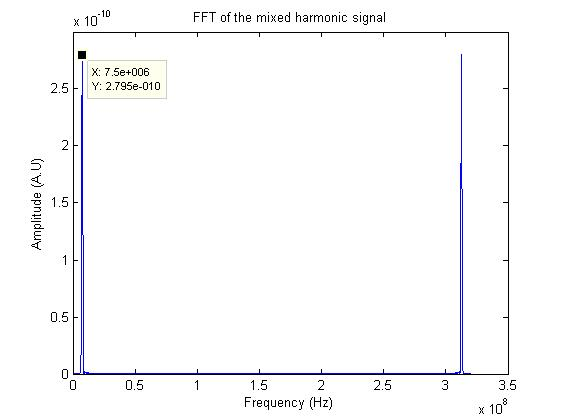
\includegraphics[scale=0.5]{images/chapter_4/finaLfft_nozzom.jpg}
\caption{FFT of generated wave}
\end{center}
\end{figure}

\begin{figure}
\begin{center}
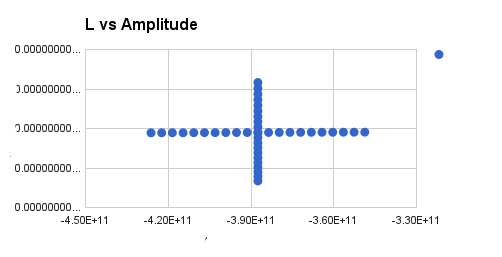
\includegraphics[scale=0.7]{images/chapter_4/lvsamp.png}
\caption{effect of l on the amplitude of generated wave}
\end{center}
\end{figure}

\begin{figure}
\begin{center}
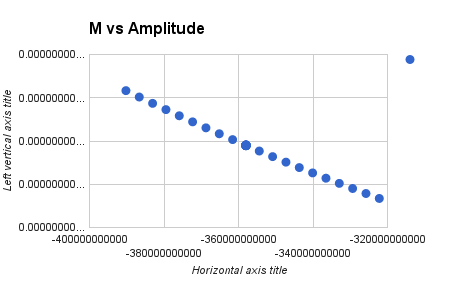
\includegraphics[scale=0.7]{images/chapter_4/mvsamp.png}
\caption{effect of m on the amplitude of generated wave}
\end{center}
\end{figure}
\section{Results and Discussion}
From the plots of amplitude of resultant wave with respect to the perturbation of constants, it is clear that amplitude changes only with changes in the value of m, and is agnostic to the value of l. One of the reasons for this could be because of the problem under consideration itself. We are working with collinear mixing where one degree of freedom is lost while waves are mixing. Another reason is the mixing of transverse and longitudinal waves result in a transverse wave which is affected only by this constant in a 2D situation. For a non-collinear approach, this would change significantly. Due to multiple interactions happening in the material.

All the resulting waves had a similar peak frequency, and thus frequency of the resultant wave wasn't used further for modelling the inverse.